\documentclass{article}

\usepackage{fancyhdr}
\usepackage{extramarks}
\usepackage{amsmath}
\usepackage{amsthm}
\usepackage{amsfonts}
\usepackage{tikz}
\usepackage[plain]{algorithm}
\usepackage{algpseudocode}
\usepackage[shortlabels]{enumitem}
\usepackage{mathtools}
\usepackage{amssymb}

\usetikzlibrary{automata,positioning}

%
% Basic Document Settings
%

\topmargin=-0.45in
\evensidemargin=0in
\oddsidemargin=0in
\textwidth=6.5in
\textheight=9.0in
\headsep=0.25in

\linespread{1.1}

\pagestyle{fancy}
\lhead{\hmwkAuthorName}
\chead{\hmwkClass\ (\hmwkClassInstructor\ \hmwkClassTime): \hmwkTitle}
\lfoot{\lastxmark}
\cfoot{\thepage}

\renewcommand\headrulewidth{0.4pt}
\renewcommand\footrulewidth{0.4pt}

\setlength\parindent{0pt}

%
% Create Problem Sections
%

\newcommand{\enterProblemHeader}[1]{
    \nobreak\extramarks{}{Problem \arabic{#1} continued on next page\ldots}\nobreak{}
    \nobreak\extramarks{Problem \arabic{#1} (continued)}{Problem \arabic{#1} continued on next page\ldots}\nobreak{}
}

\newcommand{\exitProblemHeader}[1]{
    \nobreak\extramarks{Problem \arabic{#1} (continued)}{Problem \arabic{#1} continued on next page\ldots}\nobreak{}
    \stepcounter{#1}
    \nobreak\extramarks{Problem \arabic{#1}}{}\nobreak{}
}

\setcounter{secnumdepth}{0}
\newcounter{partCounter}
\newcounter{homeworkProblemCounter}
\setcounter{homeworkProblemCounter}{1}
\nobreak\extramarks{Problem \arabic{homeworkProblemCounter}}{}\nobreak{}

\newcommand{\hmwkTitle}{Mod 3}
\newcommand{\hmwkDueDate}{March 20, 2025}
\newcommand{\hmwkClass}{Discrete Math}
\newcommand{\hmwkClassTime}{Section 001}
\newcommand{\hmwkClassInstructor}{Mark Floryan}
\newcommand{\hmwkAuthorName}{\textbf{Rushil Umaretiya}}

%
% Title Page
%

\title{
    \vspace{2in}
    \textmd{\textbf{\hmwkTitle}}\\
    \normalsize\vspace{0.1in}
    \small{\textbf{Due\ on\ \hmwkDueDate}}\\
    \normalsize\text{Tuesday/Thursday 11:00-12:15, Warner 209}\\
    \vspace{0.1in}\large{\textit{\hmwkClassInstructor\ - \hmwkClassTime}}
    \vspace{3in}
}

\author{\hmwkAuthorName\\\small{frj2ka@virginia.edu}}
\date{}

\renewcommand{\part}[1]{\textbf{\large Part \Alph{partCounter}}\stepcounter{partCounter}\\}

%
% Various Helper Commands
%

% Useful for algorithms
\newcommand{\alg}[1]{\textsc{\bfseries \footnotesize #1}}

% For derivatives
\newcommand{\deriv}[1]{\frac{\mathrm{d}}{\mathrm{d}x} (#1)}

% For partial derivatives
\newcommand{\pderiv}[2]{\frac{\partial}{\partial #1} (#2)}

% Integral dx
\newcommand{\dx}{\mathrm{d}x}

% Alias for the Solution section header
\newcommand{\solution}{\textbf{\large Solution}}

\newcommand{\unit}[1]{\section{Unit #1}}
\newcommand{\problem}[1]{\textbf{\##1}}
\newcommand{\prob}[1]{\problem{#1}}


% Probability commands: Expectation, Variance, Covariance, Bias
\newcommand{\E}{\mathrm{E}}
\newcommand{\Var}{\mathrm{Var}}
\newcommand{\Cov}{\mathrm{Cov}}
\newcommand{\Bias}{\mathrm{Bias}}

\renewcommand{\And}{\wedge}
\newcommand{\Or}{\vee}
\newcommand{\Xor}{\oplus}
\newcommand{\Not}{\neg}
\newcommand{\Implies}{\rightarrow}
\newcommand{\Iff}{\leftrightarrow}
\newcommand{\union}{\cup}
\newcommand{\intersection}{\cap}

\newcommand{\AllIntegers}{\mathbb{Z}}
\newcommand{\AllNaturals}{\mathbb{N}}
\newcommand{\AllRationals}{\mathbb{Q}}
\newcommand{\AllReals}{\mathbb{R}}
\newcommand{\AllComplexes}{\mathbb{C}}

\begin{document}

\maketitle

\pagebreak

\problem{1}

For each of the languages below, provide a context-free grammar that generates it (Note that some of these might also be regular languages, but we still want a grammar for each). For all parts, $\Sigma=\{0,1\}$:


\begin{itemize}
	\item Strings that contain exactly two 1's OR exactly two 0's
	
    $S \rightarrow A | X$\\
    \\
    $A \rightarrow 0A | 1B$\\
    $B \rightarrow 0B | 1C$\\
    $C \rightarrow 0C | \epsilon$\\
    \\
    $X \rightarrow 1X | 0Y$\\
    $Y \rightarrow 1Y | 0Z$\\
    $Z \rightarrow 1Z | \epsilon$\\
    
	\item Strings of even length that contain 1100 directly in the center (i.e., $w1100u \ | \ |w|=|u|$)
	
    $S \rightarrow T1100T$\\
    $T \rightarrow 0T | 1T | \epsilon$

	\item $ww^Ruu^R \ | \ w \in \Sigma^* \wedge u \in \Sigma^*$
	
    $S \rightarrow AA$\\
    $A \rightarrow 0A0 | 1A1 | \epsilon$
\end{itemize}
\pagebreak

\problem{2}

Draw PDAs for each of the languages in the previous exercise (note that you can draw a DFA / NFA if the language happens to be regular).

\begin{itemize}
	\item Strings that contain exactly two 1's OR exactly two 0's

    \begin{center}
        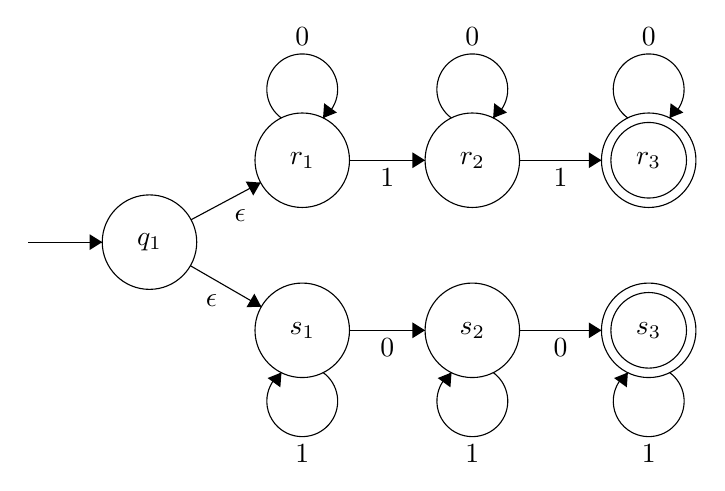
\begin{tikzpicture}[scale=0.2]
        \tikzstyle{every node}+=[inner sep=0pt]
        \draw [black] (14.9,-31.5) circle (3);
        \draw (14.9,-31.5) node {$q_1$};
        \draw [black] (24.6,-26.3) circle (3);
        \draw (24.6,-26.3) node {$r_1$};
        \draw [black] (24.6,-37.1) circle (3);
        \draw (24.6,-37.1) node {$s_1$};
        \draw [black] (35.4,-26.3) circle (3);
        \draw (35.4,-26.3) node {$r_2$};
        \draw [black] (46.6,-26.3) circle (3);
        \draw (46.6,-26.3) node {$r_3$};
        \draw [black] (46.6,-26.3) circle (2.4);
        \draw [black] (35.4,-37.1) circle (3);
        \draw (35.4,-37.1) node {$s_2$};
        \draw [black] (46.6,-37.1) circle (3);
        \draw (46.6,-37.1) node {$s_3$};
        \draw [black] (46.6,-37.1) circle (2.4);
        \draw [black] (7.2,-31.5) -- (11.9,-31.5);
        \fill [black] (11.9,-31.5) -- (11.1,-31) -- (11.1,-32);
        \draw [black] (17.54,-30.08) -- (21.96,-27.72);
        \fill [black] (21.96,-27.72) -- (21.01,-27.65) -- (21.49,-28.54);
        \draw (20.67,-29.4) node [below] {$\epsilon$};
        \draw [black] (17.5,-33) -- (22,-35.6);
        \fill [black] (22,-35.6) -- (21.56,-34.77) -- (21.06,-35.63);
        \draw (18.83,-34.8) node [below] {$\epsilon$};
        \draw [black] (23.277,-23.62) arc (234:-54:2.25);
        \draw (24.6,-19.05) node [above] {$0$};
        \fill [black] (25.92,-23.62) -- (26.8,-23.27) -- (25.99,-22.68);
        \draw [black] (27.6,-26.3) -- (32.4,-26.3);
        \fill [black] (32.4,-26.3) -- (31.6,-25.8) -- (31.6,-26.8);
        \draw (30,-26.8) node [below] {$1$};
        \draw [black] (38.4,-26.3) -- (43.6,-26.3);
        \fill [black] (43.6,-26.3) -- (42.8,-25.8) -- (42.8,-26.8);
        \draw (41,-26.8) node [below] {$1$};
        \draw [black] (34.077,-23.62) arc (234:-54:2.25);
        \draw (35.4,-19.05) node [above] {$0$};
        \fill [black] (36.72,-23.62) -- (37.6,-23.27) -- (36.79,-22.68);
        \draw [black] (27.6,-37.1) -- (32.4,-37.1);
        \fill [black] (32.4,-37.1) -- (31.6,-36.6) -- (31.6,-37.6);
        \draw (30,-37.6) node [below] {$0$};
        \draw [black] (45.277,-23.62) arc (234:-54:2.25);
        \draw (46.6,-19.05) node [above] {$0$};
        \fill [black] (47.92,-23.62) -- (48.8,-23.27) -- (47.99,-22.68);
        \draw [black] (38.4,-37.1) -- (43.6,-37.1);
        \fill [black] (43.6,-37.1) -- (42.8,-36.6) -- (42.8,-37.6);
        \draw (41,-37.6) node [below] {$0$};
        \draw [black] (25.923,-39.78) arc (54:-234:2.25);
        \draw (24.6,-44.35) node [below] {$1$};
        \fill [black] (23.28,-39.78) -- (22.4,-40.13) -- (23.21,-40.72);
        \draw [black] (36.723,-39.78) arc (54:-234:2.25);
        \draw (35.4,-44.35) node [below] {$1$};
        \fill [black] (34.08,-39.78) -- (33.2,-40.13) -- (34.01,-40.72);
        \draw [black] (47.923,-39.78) arc (54:-234:2.25);
        \draw (46.6,-44.35) node [below] {$1$};
        \fill [black] (45.28,-39.78) -- (44.4,-40.13) -- (45.21,-40.72);
        \end{tikzpicture}
    \end{center}
	\item Strings of even length that contain 1100 directly in the center (i.e., $w1100u \ | \ |w|=|u|$)
	
\begin{center}
    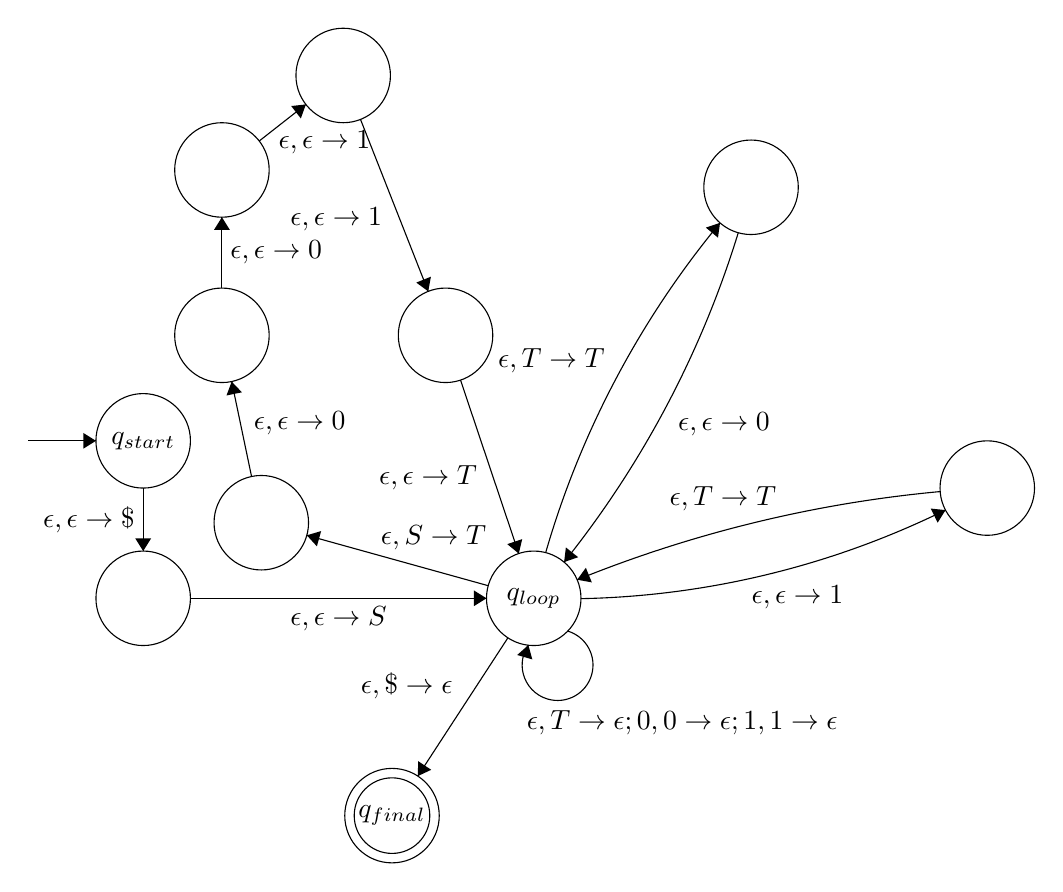
\begin{tikzpicture}[scale=0.2]
    \tikzstyle{every node}+=[inner sep=0pt]
    \draw [black] (10.3,-31.7) circle (3);
    \draw (10.3,-31.7) node {$q_{start}$};
    \draw [black] (10.3,-41.7) circle (3);
    \draw [black] (35.1,-41.7) circle (3);
    \draw (35.1,-41.7) node {$q_{loop}$};
    \draw [black] (26.1,-55.5) circle (3);
    \draw (26.1,-55.5) node {$q_{final}$};
    \draw [black] (26.1,-55.5) circle (2.4);
    \draw [black] (17.8,-36.9) circle (3);
    \draw [black] (15.3,-25) circle (3);
    \draw [black] (15.3,-14.5) circle (3);
    \draw [black] (23,-8.5) circle (3);
    \draw [black] (29.5,-25) circle (3);
    \draw [black] (48.9,-15.6) circle (3);
    \draw [black] (63.9,-34.7) circle (3);
    \draw [black] (3,-31.7) -- (7.3,-31.7);
    \fill [black] (7.3,-31.7) -- (6.5,-31.2) -- (6.5,-32.2);
    \draw [black] (10.3,-34.7) -- (10.3,-38.7);
    \fill [black] (10.3,-38.7) -- (10.8,-37.9) -- (9.8,-37.9);
    \draw (9.8,-36.7) node [left] {$\epsilon,\epsilon \rightarrow \$$};
    \draw [black] (13.3,-41.7) -- (32.1,-41.7);
    \fill [black] (32.1,-41.7) -- (31.3,-41.2) -- (31.3,-42.2);
    \draw (22.7,-42.2) node [below] {$\epsilon,\epsilon \rightarrow S$};
    \draw [black] (33.46,-44.21) -- (27.74,-52.99);
    \fill [black] (27.74,-52.99) -- (28.59,-52.59) -- (27.76,-52.04);
    \draw (29.98,-47.28) node [left] {$\epsilon, \$ \rightarrow \epsilon$};
    \draw [black] (32.21,-40.9) -- (20.69,-37.7);
    \fill [black] (20.69,-37.7) -- (21.33,-38.4) -- (21.6,-37.43);
    \draw (28.74,-38.63) node [above] {$\epsilon,S \rightarrow T$};
    \draw [black] (17.18,-33.96) -- (15.92,-27.94);
    \fill [black] (15.92,-27.94) -- (15.59,-28.82) -- (16.57,-28.62);
    \draw (17.29,-30.61) node [right] {$\epsilon,\epsilon \rightarrow 0$};
    \draw [black] (15.3,-22) -- (15.3,-17.5);
    \fill [black] (15.3,-17.5) -- (14.8,-18.3) -- (15.8,-18.3);
    \draw (15.8,-19.75) node [right] {$\epsilon,\epsilon \rightarrow 0$};
    \draw [black] (17.67,-12.66) -- (20.63,-10.34);
    \fill [black] (20.63,-10.34) -- (19.7,-10.44) -- (20.31,-11.23);
    \draw (21.81,-12) node [below] {$\epsilon,\epsilon \rightarrow 1$};
    \draw [black] (24.1,-11.29) -- (28.4,-22.21);
    \fill [black] (28.4,-22.21) -- (28.57,-21.28) -- (27.64,-21.65);
    \draw (25.5,-17.62) node [left] {$\epsilon,\epsilon \rightarrow 1$};
    \draw [black] (30.45,-27.84) -- (34.15,-38.86);
    \fill [black] (34.15,-38.86) -- (34.37,-37.94) -- (33.42,-38.26);
    \draw (31.53,-34.06) node [left] {$\epsilon,\epsilon \rightarrow T$};
    \draw [black] (35.859,-38.798) arc (163.86119:140.40481:58.255);
    \fill [black] (46.93,-17.86) -- (46.03,-18.16) -- (46.8,-18.8);
    \draw (39.64,-26.6) node [left] {$\epsilon,T \rightarrow T$};
    \draw [black] (48.087,-18.488) arc (-17.07756:-38.65645:63.191);
    \fill [black] (37.03,-39.4) -- (37.92,-39.09) -- (37.14,-38.47);
    \draw (44.23,-30.63) node [right] {$\epsilon,\epsilon \rightarrow 0$};
    \draw [black] (61.245,-36.096) arc (-63.8202:-88.85749:54.945);
    \fill [black] (61.25,-36.1) -- (60.31,-36) -- (60.75,-36.9);
    \draw (51.84,-40.87) node [below] {$\epsilon,\epsilon \rightarrow 1$};
    \draw [black] (37.859,-40.523) arc (112.04992:95.27239:81.295);
    \fill [black] (37.86,-40.52) -- (38.79,-40.69) -- (38.41,-39.76);
    \draw (47.11,-36.16) node [above] {$\epsilon,T \rightarrow T$};
    \draw [black] (37.247,-43.779) arc (73.65382:-214.34618:2.25);
    \draw (44.53,-48.78) node [below] {$\epsilon,T \rightarrow \epsilon;0,0 \rightarrow \epsilon;1,1 \rightarrow \epsilon$};
    \fill [black] (34.76,-44.67) -- (34.05,-45.3) -- (35.01,-45.58);
    \end{tikzpicture}
    \end{center}
    
    \pagebreak

    \item $ww^Ruu^R \ | \ w \in \Sigma^* \wedge u \in \Sigma^*$


\begin{center}
    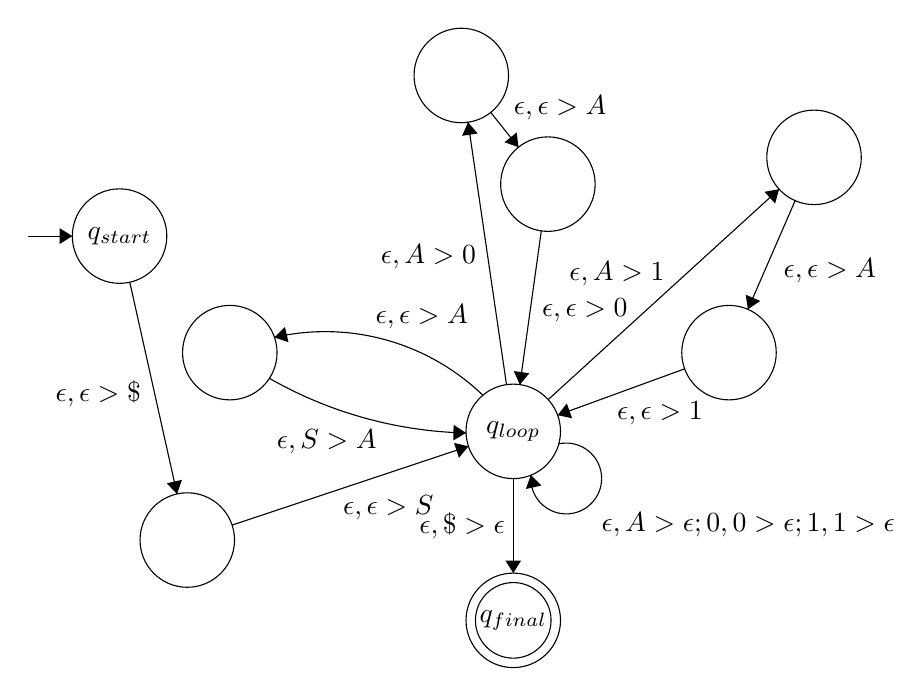
\begin{tikzpicture}[scale=0.2]
    \tikzstyle{every node}+=[inner sep=0pt]
    \draw [black] (10.3,-24.3) circle (3);
    \draw (10.3,-24.3) node {$q_{start}$};
    \draw [black] (14.6,-43.6) circle (3);
    \draw [black] (35.3,-36.7) circle (3);
    \draw (35.3,-36.7) node {$q_{loop}$};
    \draw [black] (35.3,-48.7) circle (3);
    \draw (35.3,-48.7) node {$q_{final}$};
    \draw [black] (35.3,-48.7) circle (2.4);
    \draw [black] (17.3,-31.7) circle (3);
    \draw [black] (32,-14.1) circle (3);
    \draw [black] (37.5,-21) circle (3);
    \draw [black] (54.4,-19.3) circle (3);
    \draw [black] (49,-31.7) circle (3);
    \draw [black] (4.5,-24.3) -- (7.3,-24.3);
    \fill [black] (7.3,-24.3) -- (6.5,-23.8) -- (6.5,-24.8);
    \draw [black] (10.95,-27.23) -- (13.95,-40.67);
    \fill [black] (13.95,-40.67) -- (14.26,-39.78) -- (13.29,-40);
    \draw (11.7,-34.33) node [left] {$\epsilon,\epsilon>\$$};
    \draw [black] (17.45,-42.65) -- (32.45,-37.65);
    \fill [black] (32.45,-37.65) -- (31.54,-37.43) -- (31.85,-38.38);
    \draw (27.36,-40.75) node [below] {$\epsilon,\epsilon>S$};
    \draw [black] (35.3,-39.7) -- (35.3,-45.7);
    \fill [black] (35.3,-45.7) -- (35.8,-44.9) -- (34.8,-44.9);
    \draw (34.8,-42.7) node [left] {$\epsilon,\$>\epsilon$};
    \draw [black] (20.134,-30.731) arc (102.91619:46.03559:14.425);
    \fill [black] (20.13,-30.73) -- (21.03,-31.04) -- (20.8,-30.07);
    \draw (29.49,-30.22) node [above] {$\epsilon,\epsilon>A$};
    \draw [black] (32.303,-36.802) arc (-91.31189:-119.73634:26.396);
    \fill [black] (32.3,-36.8) -- (31.51,-36.28) -- (31.49,-37.28);
    \draw (23.46,-36.52) node [below] {$\epsilon,S>A$};
    \draw [black] (34.87,-33.73) -- (32.43,-17.07);
    \fill [black] (32.43,-17.07) -- (32.05,-17.93) -- (33.04,-17.79);
    \draw (32.96,-25.58) node [left] {$\epsilon,A>0$};
    \draw [black] (33.87,-16.45) -- (35.63,-18.65);
    \fill [black] (35.63,-18.65) -- (35.52,-17.72) -- (34.74,-18.34);
    \draw (35.31,-16.13) node [right] {$\epsilon,\epsilon>A$};
    \draw [black] (37.08,-23.97) -- (35.72,-33.73);
    \fill [black] (35.72,-33.73) -- (36.32,-33.01) -- (35.33,-32.87);
    \draw (37.09,-29.02) node [right] {$\epsilon,\epsilon>0$};
    \draw [black] (37.52,-34.68) -- (52.18,-21.32);
    \fill [black] (52.18,-21.32) -- (51.25,-21.49) -- (51.93,-22.23);
    \draw (41.88,-27.51) node [above] {$\epsilon,A>1$};
    \draw [black] (53.2,-22.05) -- (50.2,-28.95);
    \fill [black] (50.2,-28.95) -- (50.98,-28.42) -- (50.06,-28.02);
    \draw (52.43,-26.47) node [right] {$\epsilon,\epsilon>A$};
    \draw [black] (46.18,-32.73) -- (38.12,-35.67);
    \fill [black] (38.12,-35.67) -- (39.04,-35.87) -- (38.7,-34.93);
    \draw (44.61,-34.77) node [below] {$\epsilon,\epsilon>1$};
    \draw [black] (38.181,-37.494) arc (102.32535:-185.67465:2.25);
    \draw (40.88,-42.64) node [right] {$\epsilon,A>\epsilon;0,0>\epsilon;1,1>\epsilon$};
    \fill [black] (36.42,-39.47) -- (36.1,-40.36) -- (37.08,-40.14);
    \end{tikzpicture}
    \end{center}

\end{itemize}

\pagebreak

\problem{3}

For this question, you will prove that context-free languages are NOT closed under intersection. The alphabet for all languages in this question is $\Sigma = \{a,b,c\}$ Do this by showing the following:

\begin{itemize}
	\item \textbf{Part 1:} First, show that $A=\{a^mb^nc^n | m,n \geq 0\}$ is context-free by producing a context-free grammar that generates it.
	
    $S \rightarrow AB $\\
    $A \rightarrow aA | \epsilon$\\
    $B \rightarrow bBc | \epsilon$

	\item \textbf{Part 2:} Do the same, but for language $B=\{a^nb^nc^m | m,n \geq 0\}$
	
    $S \rightarrow AB $\\
    $A \rightarrow aAb | \epsilon$\\
    $B \rightarrow cB | \epsilon$

	\item \textbf{Part 3:} Lastly, find the intersection of these two sets and use the pumping lemma to show that the intersection language is not context-free.
	
    $A \cap B = \{a^nb^nc^n | n \geq 0\}$\\
    \\
    Assume $A \cap B$ is context-free.\\
    Let $p$ be the pumping length.\\
    Let $s = a^pb^pc^p$.\\
    \\
    By the pumping lemma, $s$ can be divided into $s = uvwxy$ such that:
    \begin{enumerate}
        \item $|vwx| \leq p$
        \item $|vx| \geq 1$
        \item $uv^iwx^iy \in A \cap B$ for all $i \geq 0$
    \end{enumerate}

    Given $s = a^pb^pc^p$, $vwx$ must be contained in the first $p$ characters of $s$.\\
    \\
    We can divide $s$ into 2 cases:

    \begin{enumerate}
        \item $vwx$ contains only one type of character.\\
        In this case, $uv^2wx^2y$ will contain more of one type of character than the other two types.\\
        Thus, $uv^2wx^2y \notin A \cap B$.
        \item $vwx$ contains two types of characters.\\
        In this case, $uv^2wx^2y$ will make it such that the characters are out of order (a then b then c).\\
        Thus, $uv^2wx^2y \notin A \cap B$.
    \end{enumerate}

    In both cases, $uv^2wx^2y \notin A \cap B$. Thus, $A \cap B$ is not context-free.

\end{itemize}

\pagebreak

\problem{4}
Let us define a new operation using the $\Diamond$ symbol as such: if $A$ and $B$ are languages, then $A \Diamond B = \{xy | x \in A, y \in B, |x|=|y| \}$. Prove that if $A$ and $B$ are regular languages, then $A \Diamond B$ must be a context-free language.

Given that A and B are regular languages, we can construct DFAs $M_A$ and $M_B$ that accept A and B, respectively.\\
\begin{itemize}
    \item Let $M_a = (Q_a, \Sigma, \delta_a, q_{0a}, F_a)$ be the DFA that accepts $A$.
    \item Let $M_b = (Q_b, \Sigma, \delta_b, q_{0b}, F_b)$ be the DFA that accepts $B$.
\end{itemize}

Then we can construct a PDA $M$ that accepts $A \Diamond B$ as follows:

Given $P = (Q, \Sigma, \Gamma, \delta, q_0, F)$ where:

\begin{itemize}
    \item $Q = {q_0, q_{final}} \union Q_a \union Q_b$
    \item $\Gamma = \Sigma \union \{\$\}$
    \item $F = {q_{final}}$
    \item $\delta$ is defined as follows:
\end{itemize}

First, we'll push a \$ onto the stack to mark the end empty point and we'll transition to the start state of $M_a$. At each read input, we'll push a \# onto the stack in order to keep track of the length of $x$. Then at every accept state for $M_a$ we'll perform a $\epsilon$ transition to the start state of $M_b$. At each read input and during this epsilon transition, we'll pop a \# from the stack in order to keep track of the length of $y$. Then at every accept state for $M_b$ we'll perform a $\epsilon$ transition to the final state. If the stack is empty (i.e., there is a \$ remaining) and we're at the final state, we'll accept the string.

This PDA would look something like this with augmented $M_a$ to push on every transition and $M_b$ to pop on every transition:


\begin{center}
    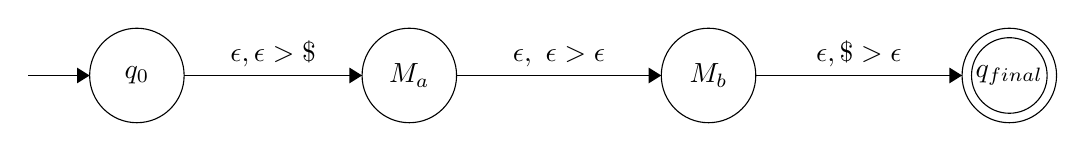
\begin{tikzpicture}[scale=0.2]
    \tikzstyle{every node}+=[inner sep=0pt]
    \draw [black] (9.2,-32.3) circle (3);
    \draw (9.2,-32.3) node {$q_0$};
    \draw [black] (26.5,-32.3) circle (3);
    \draw (26.5,-32.3) node {$M_a$};
    \draw [black] (45.5,-32.3) circle (3);
    \draw (45.5,-32.3) node {$M_b$};
    \draw [black] (64.6,-32.3) circle (3);
    \draw (64.6,-32.3) node {$q_{final}$};
    \draw [black] (64.6,-32.3) circle (2.4);
    \draw [black] (2.3,-32.3) -- (6.2,-32.3);
    \fill [black] (6.2,-32.3) -- (5.4,-31.8) -- (5.4,-32.8);
    \draw [black] (12.2,-32.3) -- (23.5,-32.3);
    \fill [black] (23.5,-32.3) -- (22.7,-31.8) -- (22.7,-32.8);
    \draw (17.85,-31.8) node [above] {$\epsilon,\epsilon>\$$};
    \draw [black] (29.5,-32.3) -- (42.5,-32.3);
    \fill [black] (42.5,-32.3) -- (41.7,-31.8) -- (41.7,-32.8);
    \draw (36,-31.8) node [above] {$\epsilon,\mbox{ }\epsilon>\epsilon$};
    \draw [black] (48.5,-32.3) -- (61.6,-32.3);
    \fill [black] (61.6,-32.3) -- (60.8,-31.8) -- (60.8,-32.8);
    \draw (55.05,-31.8) node [above] {$\epsilon,\$>\epsilon$};
    \end{tikzpicture}
    \end{center}

This PDA recognizes $A \Diamond B$ because it ensures $x \in A$ by simulating $M_a$ and $y \in B$ by simulating $M_b$ and ensures that $|x| = |y|$ by pushing a \# for every character in $x$ and popping a \# for every character in $y$. Since PDAs recognize exactly the context-free languages, and we've constructed a PDA that recognizes $A \Diamond B$, we've shown that $A \Diamond B$ is a context-free language.

\pagebreak

\problem{5}
Suppose you have a context-free language $C$ and a regular language $R$. Prove that $C \cap R$ is context-free.

Given a PDA $P$ that recognizes $C$, we can just use the DFA $D$ that recognizes $R$ to simulate the PDA $P$. We can construct a new PDA $P'$ that recognizes $C \cap R$ as follows by simulating $P$ and $D$ in parallel:\\
\\
Given $P = (Q_p, \Sigma, \Gamma_p, \delta_p, q_{0p}, F_p)$ and $D = (Q_d, \Sigma, \delta_d, q_{0d}, F_d)$, build $P' = (Q, \Sigma, \Gamma, \delta, q_0, F)$ where:

\begin{itemize}
    \item $Q = Q_p \times Q_d$
    \item $\Gamma = \Gamma_p$
    \item $F = F_p \times F_d$
    \item $\delta$ is defined as follows:
\end{itemize}
\begin{center}
    For each transition in $P$ where $\delta_p(q,a,X) = (p,Y)$, and each transition in $D$ where $\delta_d(r,a) = s$:
    \begin{align*}
        \delta((q,r),a,X) = ((p,s),Y)
    \end{align*}
\end{center}

Since we are able to construct a PDA for $C \cap R$, we have shown that $C \cap R$ is a context-free language and that the intersection of a CFL and RL is context-free.

\pagebreak

\problem{6}
Consider the language $A = \{w \ | \ w \in \{a,b,c\}^* \wedge F(w,a) = F(w,b) = F(w,c)\}$ where $F(w,a)$ counts the number of occurences of character $a$ in string $w$. Prove that $A$ is not context-free by using the result of the previous question (\emph{Hint: Assume this language is a CFL and intersect it with a regular language of your choice!})

We'll conduct a proof by contradiction. Assume that $A$ is a context-free language.\\
\\
Given the results of the previous question we can intersect $A$ with the regular language $B = a^*b^*c^*$ to get $A \cap B$ = ${a^nb^nc^n | n \geq 0}$.\\

Now, we've already shown in problem 3, part 3 that due to the pumping lemma that $A \cap B$ is not context-free. This proof has been provided again below.\\
\\
Assume $A \cap B$ is context-free.\\
Let $p$ be the pumping length.\\
Let $s = a^pb^pc^p$.\\
\\
By the pumping lemma, $s$ can be divided into $s = uvwxy$ such that:
\begin{enumerate}
    \item $|vwx| \leq p$
    \item $|vx| \geq 1$
    \item $uv^iwx^iy \in A \cap B$ for all $i \geq 0$
\end{enumerate}

Given $s = a^pb^pc^p$, $vwx$ must be contained in the first $p$ characters of $s$.\\
\\
We can divide $s$ into 2 cases:

\begin{enumerate}
    \item $vwx$ contains only one type of character.\\
    In this case, $uv^2wx^2y$ will contain more of one type of character than the other two types.\\
    Thus, $uv^2wx^2y \notin A \cap B$.
    \item $vwx$ contains two types of characters.\\
    In this case, $uv^2wx^2y$ will make it such that the characters are out of order (a then b then c).\\
    Thus, $uv^2wx^2y \notin A \cap B$.
\end{enumerate}

In both cases, $uv^2wx^2y \notin A \cap B$. Thus, $A \cap B$ is not context-free. Given that $A \cap B$ is not context-free, we have shown that $A$ is not context-free as CFLs are closed under intersection with RLs.

\pagebreak

\problem{7}

Prove that the language $A$ from the previous question is not context-free again, but this time do so by utilizing the \emph{Pumping Lemma for Context-Free Languages}.\\
\\
We can solve this problem purely using the pumping lemma for context-free languages through a proof by contradiction. If A is context-free, then there exists a pumping length p $\geq$ 1 such that any string s $\in$ A with $|s| \geq p$ can be divided into five strings $s = uvwxy$ such that:
\begin{enumerate}
    \item $uv^iwx^iy \in A$ for all $i \geq 0$
    \item $|vx| \geq 1$
    \item $|vwx| \leq p$
\end{enumerate}

Consider the string $s = a^pb^pc^p$. Since $|s| \geq p$, we can apply the pumping lemma to $s$. Since the substring $vwx$ must be contained in the first $p$ characters of $s$, $vwx$ cannot contain all three characters $a$, $b$, and $c$. This leaves us with the following two cases:

\begin{enumerate}
    \item $vwx$ contains only one type of character.\\
    In this case, we will end up with more of one type of character than the other two types when we pump $v$ and $x$. Thus, $uv^2wx^2y \notin A$.
    \item $vwx$ contains two types of characters.\\
    In this case, we will end up with the characters out of order (a then b then c) when we pump $v$ and $x$. Thus, $uv^2wx^2y \notin A$.
\end{enumerate}

In all cases, we have shown that there exists some value of $i$ such that $uv^iwx^iy \notin A$. Thus, contradicting the first condition of the pumping lemma. Since assuming that A is context-free leads to a contradiction, we have shown that A is not context-free.

\end{document}